% !Mode:: "TeX:UTF-8"
% !TEX program  = xelatex
% !BIB program  = biber
\documentclass[AutoFakeBold,AutoFakeSlant,scheme=plain,degree=bachelor,zihao=-4]{sustechthesis}
% 1. AutoFakeBold 与 AutoFakeSlant 为伪粗与伪斜,如果本机上有相应粗体与斜体字体,请使用 xeCJK 宏包进行设置,例如:
%   \setCJKmainfont[
%     UprightFont = * Light,
%     BoldFont = * Bold,
%     ItalicFont = Kaiti SC,
%     BoldItalicFont = Kaiti SC Bold,
%   ]{Songti SC}
%
% 2. scheme=chinese 为 ctexart 文类提供的中文排版方案,如果使用英文进行论文创作,请使用 scheme=plain 选项。
%
% 3. degree=bachelor 为 sustechthesis 文类提供的本科生毕业论文模板,其他可选项为 master 与 doctor,但是均未实现,如果您对此有兴趣,欢迎 PR。
%
% 4. sustechthesis.cls 文类主要参考自去年完成使命的 sustechthesis.tex,在这一年的时间,作者的 TeX 风格与常用宏包发生许多变化,因为之前的思想为仅提供必要的格式修改相关代码,所以转换为文类形式所进行的修改较少,而近期的风格与常用宏包均体现在以下的例子文件中。
%
% 5. 示例文件均放置于相应目录的 examples 文件夹下,构建自己论文时可暂时保留,用以检索接口与使用方法。
%
% 6. 英文目录需要居中可以使用:\renewcommand{\contentsname}{\centerline{Content}}
%
% 7. LaTeX 中公式编号括号样式及章节关联的方法:https://liam.page/2013/08/23/LaTeX-Formula-Number/

% !Mode:: "TeX:UTF-8"
% !TEX program  = xelatex

% 数学符号与环境
\usepackage{amsmath,amssymb}
  \newcommand{\dd}{\mathrm{d}}
  \newcommand{\RR}{\mathbb{R}}
% 参考文献
% \usepackage[style=gb7714-2015]{biblatex}
  % \addbibresource{ref.bib}
  % \usepackage{biblatex}
\usepackage{cite}
% 无意义文本
\usepackage{zhlipsum,lipsum}
% 列表环境设置
\usepackage{enumitem}
% 浮动题不越过 \section
\usepackage[section]{placeins}
% 超链接
\usepackage{hyperref}
% 图片,子图,浮动题设置, 表格
\usepackage{graphicx,subcaption,float}
\usepackage{booktabs}
\usepackage{multirow}
\usepackage{graphicx}
\usepackage[figuresright]{rotating}
% 抄录环境设置,更多有趣例子请命令行输入 `texdoc tcolorbox`
\usepackage{tcolorbox}
  \tcbuselibrary{xparse}
  \DeclareTotalTCBox{\verbbox}{ O{green} v !O{} }%
    {fontupper=\ttfamily,nobeforeafter,tcbox raise base,%
    arc=0pt,outer arc=0pt,top=0pt,bottom=0pt,left=0mm,%
    right=0mm,leftrule=0pt,rightrule=0pt,toprule=0.3mm,%
    bottomrule=0.3mm,boxsep=0.5mm,bottomrule=0.3mm,boxsep=0.5mm,%
    colback=#1!10!white,colframe=#1!50!black,#3}{#2}%
\tcbuselibrary{listings,breakable}
  \newtcbinputlisting{\Python}[2]{
    listing options={language=Python,numbers=left,numberstyle=\tiny,
      breaklines,commentstyle=\color{white!50!black}\textit},
    title=\texttt{#1},listing only,breakable,
    left=6mm,right=6mm,top=2mm,bottom=2mm,listing file={#2}}
% 三线表支持
\usepackage{booktabs}

% LaTeX logo
\usepackage{hologo}

\usepackage{multicol}
 % 导言区
% !Mode:: "TeX:UTF-8"
% !TEX program  = xelatex
\设置信息{
    % 键 = {{中文值}, {英文值}},
    分类号 = {{}, {}},
    编号 = {{}, {}},
    UDC = {{}, {}},
    密级 = {{}, {}},
    % 仅题目(不含副标题)、系别、专业,支持手动 \\ 换行,不支持自动换行。
    题目 = {{在Hive上实现基于学习的优化器}, {An Learning-Based Optimizer\\for Hive}},
    % 如无需副标题,删除值内容即可,不可删除键定义。
    副标题 = {{}, {}},
    姓名 = {{李奇隆}, {Qilong Li}},
    学号 = {{11811410}, {11811410}},
    系别 = {{计算机科学与工程系}, {Department of Computer Science\\and Engineering}},
    专业 = {{计算机科学与技术}, {Computer Science and Technology}},
    指导老师 = {{唐博}, {Bo~Tang}},
    时间 = {{22年3月30日}, {March 30, 2022}},
    职称 = {{助理教授}, {Assistant Professor}},
}
 % 论文信息
\begin{document}

% \中文标题页\英文标题页
% \中文诚信承诺书\英文诚信承诺书
\英文标题页
\英文诚信承诺书
\摘要标题
% !Mode:: "TeX:UTF-8"
% !TEX program  = xelatex
\begin{英文摘要}{Query Optimizer, Machine Learning, Distributed System, Hive}
    Cost and cardinality estimation is vital to query optimizer, which can guide the query plan selection. However traditional
    empirical cost and cardinality estimation techniques cannot provide high-quality estimation, because they may not effectively 
    capture the correlation between multiple tables. Recently the database community shows that the learning-based cardinality 
    estimation is better than the empirical methods. However, all of these work takes standalone database as the experiment environment.
    In this work, we plan to implement a learning-based query optimizer in a distributed data warehouse, hive.
\end{英文摘要}

% \begin{中文摘要}{\LaTeX ;接口}
% 笔者见到的毕业论文模板,大多是以文类的形式,少部分以宏包的形式,并且在模板中大多掺杂着各式各样的例子(除了维护频率高的模板),导致模板文件使用了大部分与形式格式不相关的内容,代码量巨大文档欠缺且不容易修改,出现问题需要查看宏包或者文类的源代码。于是,秉着仅提供实现最基本要求的理念,重构了之前所写的 \TeX\ 形式。由于第二年使用该模板,所以设计出的模板接口不能保证以后不发生重大变动,一切以文档为主。毕竟学校在发展初期,各类文件都在日渐完善,前几年时,学校标志及名称还发生变化,同时毕业论文的样式也发生了重大变化。但是可以保证的是,模板提供的接口均为中文形式\footnote{使用 \hologo{XeLaTeX} 特性,一方面增加辨识度,另一方面不拘泥于英文命名的规则。当然此举也有些许弊端,在此就不过多展开。},并且至少更新到 2021 年,也就是笔者毕业。模板这种东西不能保证一劳永逸,一方面学校的标准制度都在发生着改变,另一方面 \hologo{LaTeX} 的宏包也在发生着改变,早先流行的宏包可能几年后就被“淘汰”掉。因此,您的使用与反馈是我不断更新的动力,希望各位不吝赐教。
% \end{中文摘要}


 % 论文摘要

\目录\clearpage % 目录及换页

\section{Introduction}
    \paragraph{}
    Optimizer is a critical component of a database system as it can optimize query execution plan to reduce database
    system execution time based on data and system metrics. Inside the optimizer, cardinality and cost estimation play 
    an important role in the optimization. Traditional cost estimation and cardinality estimation are based on rules, 
    which cannot take into account the relations between tables and columns in database instances. As a result, the 
    estimation results are very inaccurate, which caused the optimizer can not select the optimal execution plan. 
    \paragraph{}
    In recent years, there have been many works
    \cite{marcus2019neo, yang2020neurocard,wu2021unified,yang2019deep,sun2019end} on the application of learning model 
    to database system optimization, especially the application of learning model to the optimization of cardinality 
    estimation which have greatly improved the accuracy of estimation results. However, most of the current works remain 
    at the level of cardinality estimation\cite{marcus2019neo, yang2020neurocard,wu2021unified,yang2019deep}, 
    and the improvement indicators are the improvement of estimation errors. There is few work\cite{sun2019end} 
    foucs on whether the optimized estimation improves the performance of the data system. In 
    addition, all of these works take the stand-alone database instance as the test environment and threr is no  
    corresponding work for the distributed data system which is widely used and in urgent need of performance improvement.
    Based on these two problems, we plan to design and implement a learning-based query optimizer and integerate it to 
    hive\cite{Hive}, which is a well known data warehouse software project and widely used in industry.

\section{Related Work}
    In this part, we review works that are most relevant to ours.
    \subsection{Traditional Cardinality Estimator}
    \paragraph{}
    \emph{Histogram-based} cardinality estimation methods\cite{Self-Tuning-Histograms} have been widely used in many 
    industrial database systems as they are simple and have very low overhead. However, they lack the ability to capture 
    the data correlations among the tables as they make the attribute-value-independence assumption. 
    \emph{Sampling-based} approaches\cite{Two-Level-Sampling} outperform histogram-based methods as the correlations 
    in data are naturally captured by data samples. However, sampling-based approaches have two limitations: (i) empty 
    sampling set of join result; and (ii) high sampling overhead. Recent works have proposed index-based and 
    materialized sampling strategies to alleviate the problem of empty result. However, it is still difficult to use 
    sampling to evaluate the cost of all execution plans as it incurs high space- and time- costs.
    
    \subsection{Learning-Based Cardinality Estimator}
    \paragraph{}
    Recently, the database community recognized the potential of replacing traditional cardinality estimation methods 
    by learning-based models (e.g., neural network, autoregressive model)\cite{Lan2021ASO}. Existing learning-based 
    estimators can be classified into three categories: query-driven, datadriven and hybrid.
    \paragraph{}
    \textbf{Data-driven} cardinality estimators\cite{yang2019deep, yang2020neurocard} share the same idea with traditional 
    cardinality estimation methods, i.e., they hope to capture the correlations and distributions of data across the 
    tables. DeepDB\cite{yang2019deep} adopts relational sum product networks (RSPN) to capture the probability 
    distribution among relations, and translates a query into the evaluations of probabilities and expectations based 
    on RSPN. Naru\cite{naru2019} adopts autoregressive models, i.e., masked autoencoder and transformer to estimate 
    the selectivity of equal and range predicates. NeuroCard\cite{yang2020neurocard} trains a single deep autoregressive 
    model based on samples collected from the full outer join result of all relations. The model can be used to answer 
    complex queries with joins on any subset of the relations. 
    \paragraph{}
    \textbf{Query-driven} cardinality estimators\cite{deeplearningmodel20,sun2019end} formulate cardinality estimation as a 
    regression problem. The contents of queries and their true cardinalities are used as training data to learn a 
    mapping from queries to cardinalities. MSCN\cite{kipf2018learned} transforms a query into a feature vector and 
    uses a multi-set convolution network to map it to cardinality estimation. TLSTM processes a query execution plan
    recursively following its tree structure using LSTM (a kind of RNN).
    \paragraph{}
    \textbf{Hybrid} cardinality estimator UAE\cite{wu2021unified} learns the joint data distribution among the tables as in 
    the data-driven estimators, and uses query samples as auxiliary information at the same time. With a unified deep 
    autoregressive model, UAE learns from data in an unsupervised manner and query samples in a supervised manner. 

\section{Overview of Our Solution}
    \paragraph{}
    We aim to design a learning model to do cost and cardinality estimation like \cite{sun2019end} to reach end-to-end performance gain 
    in hive\cite{Hive}. We plan to choose a query-driven cardinality and cost estimation method in our learnig model, which 
    is because data-driven methods will bring a heavy overhead to data processing system because learning model based on 
    data-driven method will take much more time to train model and do reference than query-driven method while these data 
    processing systems already have a heavy workload. This work can be divided into three main tasks.
    \subsection{Design Learning Model for Estimation}
    \textbf{Feature Encoding}: Design how to extract features from query and input features into learning model.\\
    \textbf{Model Selection}: Select a suitable model, including RNN, tree convolution network, graph neural network and 
    automatic reinforcement learning model.
    \subsection{Implement Learning Model}
    \textbf{Implement Model}: Implement learning model based on design.\\
    \textbf{Train Model}: Generate trainning data collection and train the model. 
    \subsection{Integrate Learning Model into Hive}
    \textbf{Read Hive's Code}: Read sourcecode of hive query engine and learn how hive translates a SQL query into a physical 
    execution plan and how to optimize it during the transformation, which is the most time-consuming in all tasks.\\     
    \textbf{Integrate Model}: Integrate Our implemented learning model into hive and acheive an end-to-end performance gain
    in some classical benchmarks, such as JOB, TPC-DS and TPC-H.
\section{Completed Work}
    \paragraph{}
    So far, I have read most of sourcecode related to query transformation and query optimization of hive query engine which
    is the fundamental work to implement a learning-based optimizer in hive. The main content of this report is Query 
    Transformation and Query Optimization in hive query engine.
    \subsection{Query Transformation in Hive Query Engine}
        \paragraph{}
        We first foucs on the transformation of query in hive query engine. To meet users' habits in traditional standalone 
        database system, hive supports users run sql to process and access data in a distributed system. As the interface 
        between the database system and user, SQL will be converted to a physical execution plan which can be recoginized
        by execution engine before execution. Figure 1, which is from paper of hive, indicates the transformation of query.
        \begin{figure}[htb]
            \centering
            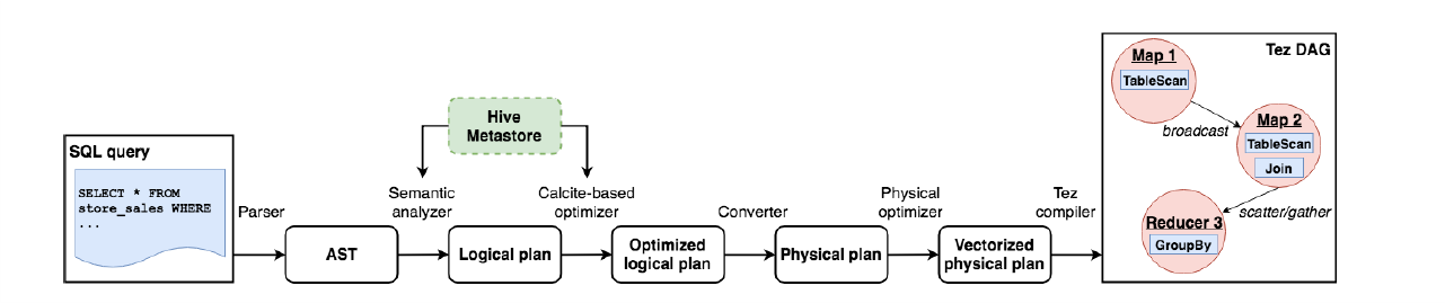
\includegraphics[width=1\textwidth]{figures/hive_mloptimizer/query_transformation.png}
            \caption{Query preparation stages in HiveServer2\cite{Hive}.}
            % 图片的标题应该在下方
        \end{figure}
        \paragraph{}
        This diagram illustrates the transformation of query in hive query engine abstractly. Let's take a look at the 
        physical implementation of each stage in code level. We take SSB\cite{ssb} Q1.1 as the experiment query.
        \paragraph*{SSB Q1.1}
        \begin{lstlisting}[language={SQL},%frame=shadowbox,    
            keywordstyle=\color{blue!30!black},  
            basicstyle=\ttfamily]  
        select 
            sum(lo_extendedprice*lo_discount) as revenue
        from 
            lineorder, dates
        where 
            lo_orderdate = d_datekey
            and d_year = 1993
            and lo_discount between 1 and 3
            and lo_quantity < 25;
        \end{lstlisting} 
        \paragraph{}
        At first, SQL is parsed as an abstract tree.
        \paragraph*{ASTree}
        \begin{lstlisting}[language={},%frame=shadowbox,    
            keywordstyle=\color{blue!30!black},  
            basicstyle=\ttfamily]  
(tok_query 
    (tok_from (tok_join 
        (tok_tabref (tok_tabname lineorder)) 
        (tok_tabref (tok_tabname dates)))
    ) 
    (tok_insert 
        (tok_destination (tok_dir tok_tmp_file)) 
        (tok_select (tok_selexpr (tok_function sum 
            (* 
                (tok_table_or_col lo_extendedprice) 
                (tok_table_or_col lo_discount)
            )) revenue)
        ) 
        (tok_where (and (and (and 
                (= 
                    (tok_table_or_col lo_orderdate) 
                    (tok_table_or_col d_datekey)
                ) 
                (= (tok_table_or_col d_year) 1993 )
            ) 
            (tok_function between kw_false 
                (tok_table_or_col lo_discount) 1 3)) 
            (< (tok_table_or_col lo_quantity) 25))
        )
    )
)
        \end{lstlisting}
        \paragraph{}
        Abstract Tree will be translated into an operator tree which is marked as logical plan in figure 1 by 
        Semantic Analyzer. Each node in the operator tree is an operator. Table scan short for TS,  which is 
        the operation that fetches data from a table, is always be the top nodes of a operator tree. This 
        logical plan has two tablse scan operator as top nodes and two branches merge in the operator JOIN[8]. 
        The merged branch ends at  the final file sink operator FS[15].
        \paragraph*{Logical plan}
        \begin{lstlisting}[language={SQL},%frame=shadowbox,    
            keywordstyle=\color{blue!30!black},  
            basicstyle=\ttfamily]  
    TS[0] - FIL[1] - SEL[2] - RS[6] - JOIN[8] - SEL[9] - SEL[10] - 
GBY[11] - RS[12] - GBY[13] - SEL[14] - FS[15]
    TS[3] - FIL[4] - SEL[5] - RS[7] - JOIN[8]
        \end{lstlisting}
        \paragraph{}
        Logical plan will be optimized by Calcite-based optimizer. With an operator tree, Optimizer will 
        match nodes of operator tree with many rewriting rules and rewrite matched nodes. Some of the classic
        rewriting rules are PredicatePushDown and JoinReorder. Optimized logical plan is following:
        \paragraph*{Optmized Logical plan}
        \begin{lstlisting}[language={SQL},%frame=shadowbox,    
            keywordstyle=\color{blue!30!black},  
            basicstyle=\ttfamily]  
    TS[0] - FIL[18] - SEL[2] - RS[6] - JOIN[8] - SEL[9] - GBY[11] - 
RS[12] - GBY[13] - FS[15]
    TS[3] - FIL[19] - SEL[5] - RS[7] - JOIN[8]
        \end{lstlisting} 
        \paragraph{}
        Comparing logical plan and optimized logical plan, we can see that FIL[1] and FIL[4] is replaced by 
        FIL[18] and FIL[19], redundant SEL[10] and SEL[14] are removed. Optimized logical plan will be converted
        into physical plan and DAG which are similar and we just show the summary graph of DAG.
        \paragraph*{DAG}
        \begin{lstlisting}[language={SQL},%frame=shadowbox,    
            keywordstyle=\color{blue!30!black},  
            basicstyle=\ttfamily]  
    Map 1 <- Map 3 (BROADCAST_EDGE)
    Reducer 2 <- Map 1 (CUSTOM_SIMPLE_EDGE)
        \end{lstlisting} 
        \paragraph{}
        In this DAG, node Map 1 and Map 3 will fetch data respectively from table lineorder and dates then 
        do filtering operation. Once Map 3 finished processing data, it will broadcast data to node Map 1. 
        Map 1 will do join and aggregate operation when it gets data from node Map 3 and send the result to 
        node Reducer 2. Reducer 2 will write the result to hdfs. Here we have explained the query's transformation 
        in hive query engine at the code level. Next, we will explain a more import issue in database system which 
        is query optimizaiton.

    \subsection{Query Optimization in Hive Query Engine}
        \paragraph{}
        Hive implements rule based optmizer(RBO) and cost based optimizer(CBO) in the query optimizer. Rule based 
        optimizer optimizes query execution plan based on defined rules while cost based optimizer optimizes query execution 
        plan based on the estimation of cost for different execution plan. Cardinality estimation is the foundation of 
        rule based optimizaiton and cost based optimizaiton because cardinality is needed to match rules in RBO and estimate 
        cost in CBO. Therefore, in this part, we will explain cardinality estimation, rule based optimizaiton and costs based 
        optimizaiton of hive query engine.
        \subsubsection{Cardinality Estimation}
            \paragraph{}
            Cardinality estimation is to estimate the row count and size of output of intermediate operators which has a great
            effect on the optimizaiton for execution plan. For instance, rule based optimizer will reorder join based on the 
            row count and size of the two tables to join. Both of RBO and CBO will select suitable join algorithm based on 
            the cardinality of two tables. Only two operators needs to perform cardinality estimation, they are the
            join operator and filter operator. Cardinality estimation of filetr operator can always reach a high accuracy 
            while join operators can not reach a stable accurate estimation because rule based cardinalities estimation lacks 
            the ability to capture the data correlations among the tables as they make the attribute-value-independence 
            assumption. Here we will explain the cardinality estimation methods for filter and join operators in hive while
            these methods is referred to \textit{Database Systems: The Complete Book}\cite{DatabaseSystems}.\\

            \textbf{Filter Operator}: Based on the assumption of uniform distribution of data\cite{DatabaseSystems}, cardinality 
            estimation result of equality comparison is the row count of table divided by the number of distinct value in the key 
            column. Assuming \textit{R} as a table, \textit{x} as the column to do filtering, \textit{T(R)} as the row count of 
            table, \textit{V(R,x)} as the number of distinct value of column \textit{x} and \textit{S} as the result table, 
            the result of cardinality estimation is $$T(S) = T(R) / V(R,x).$$For inequality comparison, based on the assumption
            that queries involving an inequality tend to retrieve a small fraction of the possible tuples and the typical
            inequality will return about one third of the tuples\cite{DatabaseSystems}, the result is $$T(S) = T(R) / 3.$$   
            
            \textbf{Join Operator}: For join operator, we assume a simple join of two tables invloves only the equality of two 
            columns and a more complicated join case can be drawn from this example. Assuming \textit{X}, \textit{Y} as two tables
            to join and \textit{x}, \textit{y} as key columns of \textit{X}, \textit{Y} to join. The cardinality estimation result
            is $$T(S) = T(X)T(Y) / max(V(X,x), V(Y,y)).$$
        \subsubsection{Rule Based Optimizer}
            \paragraph{}
            Rule based optimizer in hive optimizes execution plan based on defined rules which include rewriting rules and other rules. 
            Firstly, rule based optimizer uses defined rewriting rules to match operator tree and rewrites matched operators iteratively 
            until no rewriting in last iteration. Rewriting rule can help optimizer do many basic but important optimizaitons, such
            as FilterPushDown, JoinReorder and removing redundant operators. In addition to the rewriting rules, rule based optimizer
            also uses rules to do more like selecting the join algorithm for each join operator. Hive implements two fundamental join algorithms 
            which are Map Join and Sort Merge Join while Map Join is used when any one of join tables is a small table, otherwise, sort 
            Merge Join is used. The boundary between a big table and a small table in hive is 10MB size which is modifiable.   
        \subsubsection{Cost Based Optimizern} 
            \paragraph{}
            Similar to rule based optimizer, cost based optimizer also uses rewriting rules to do basic optimization. What makes 
            cost based optimizer different is that it computes a cost for each feasible execution plan in terms of CPU usage, IO usage, 
            cardinality and size of tuple and select the plan with least cost as the final execution plan. Unlike RBO chooses join algorithm
            only based on the sizes of join tables, CBO estimates cardinalities, CPU costs and IO cost of Map Join and Merge Join and select the
            algorithm with less total cost. 
    \paragraph{}
    In this part, we first explain the query transformation in five stages at code level and then introduce query optimization from cardinality 
    estimation, rule based optimizer and cost based optimizer, which is a simple introduction to hive query engine. So far, we have completed 
    probably the most time-consuming part of the job. Next, let's move on to future work arrangements.

\section{Work Scheduling}
    According to the remaining time to complete the graduate thesis, I had made the following schedule as table 1.
    \begin{table}[h]
        \centering
        \resizebox{\textwidth}{!}{%
        \begin{tabular}{|l|l|}
        \hline
        Date Range              & Work Arrangement                              \\ \hline
        2022.04.01 - 2022.04.10 & Design learning model                         \\ \hline
        2022.04.11 - 2022.04.20 & Implement learning model and train model      \\ \hline
        2022.04.21 - 2022.04.30 & Integrate learning model into hive           \\ \hline
        2022.05.01 - 2022.05.10 & Run expriment in hive with learning optimizer \\ \hline
        2022.05.11 - 2022.05.20 & Complete graduation thesis                    \\ \hline
        \end{tabular}%
        }
        \caption{Work Scheduling}
        \end{table}\clearpage

%\input{sections/examples/disclaimer.tex}
% \input{sections/examples/interface.tex}
% \input{sections/examples/details.tex}
% \input{sections/examples/figures.tex}
% \input{sections/examples/tutorial.tex}\clearpage
% \参考文献
%   \printbibliography[heading=none]
%   \clearpage
% \附录
%   % !Mode:: "TeX:UTF-8"
% !TEX program  = xelatex
\section*{数据获取函数}\label{A:data}
\SQL{utils.py}{code/hive_mloptimizer/ssb_Q1.1.sql}

(tok_query 
    (tok_from (tok_join 
        (tok_tabref (tok_tabname lineorder)) 
        (tok_tabref (tok_tabname dates)))
    ) 
    (tok_insert 
        (tok_destination (tok_dir tok_tmp_file)) 
        (tok_select (tok_selexpr (tok_function sum 
            (* 
                (tok_table_or_col lo_extendedprice) 
                (tok_table_or_col lo_discount)
            )) revenue)
        ) 
        (tok_where (and (and (and 
                (= 
                    (tok_table_or_col lo_orderdate) 
                    (tok_table_or_col d_datekey)
                ) 
                (= (tok_table_or_col d_year) 1993 )
            ) 
            (tok_function between kw_false 
                (tok_table_or_col lo_discount) 1 3)) 
            (< (tok_table_or_col lo_quantity) 25))
        )
    )
)

%   \clearpage
% \致谢
%   % !Mode:: "TeX:UTF-8"
% !TEX program  = xelatex
% \sustechthesis\ 目前版本为 \version, \LaTeX\ 毕业论文模板项目从提出到现在已有两年了。感谢为本项目贡献代码的开发人员们:
% \begin{itemize}
%     \item 梁钰栋(南方科技大学,本科 17 级);
%     \item 张志炅(南方科技大学,本科 17 级)。
% \end{itemize}
% 以及使用本项目,并提出诸多宝贵的修改意见的使用人员们:
% \begin{itemize}
%     \item 李未晏(南方科技大学,本科 15 级);
%     \item 张尔聪(南方科技大学,本科 15 级)。
% \end{itemize}

% 此外,目前的维护者并非计算机系,可能存在对协议等的错误使用,如果你在本模板中发现任何问题,请在 GitHub 中提出 \href{https://github.com/Iydon/sustechthesis/issues}{Issues},同时也非常欢迎对代码的贡献!

\bibliographystyle{IEEEtran}  %格式
\bibliography{ref}  %bib文件名
\end{document}


